\section{Título de la Segunda sección}
Contenido de la segunda sección. Primera bibliografia:\cite{bib2}

 \subsection{Título de la primera subsección}
Contenido de la primer subsección. La figura 1 es un ejemplo de una Figura \ref{imagen2}.

\begin{figure}[!h] %Ambiente para figuras, here.
    \begin{center}
        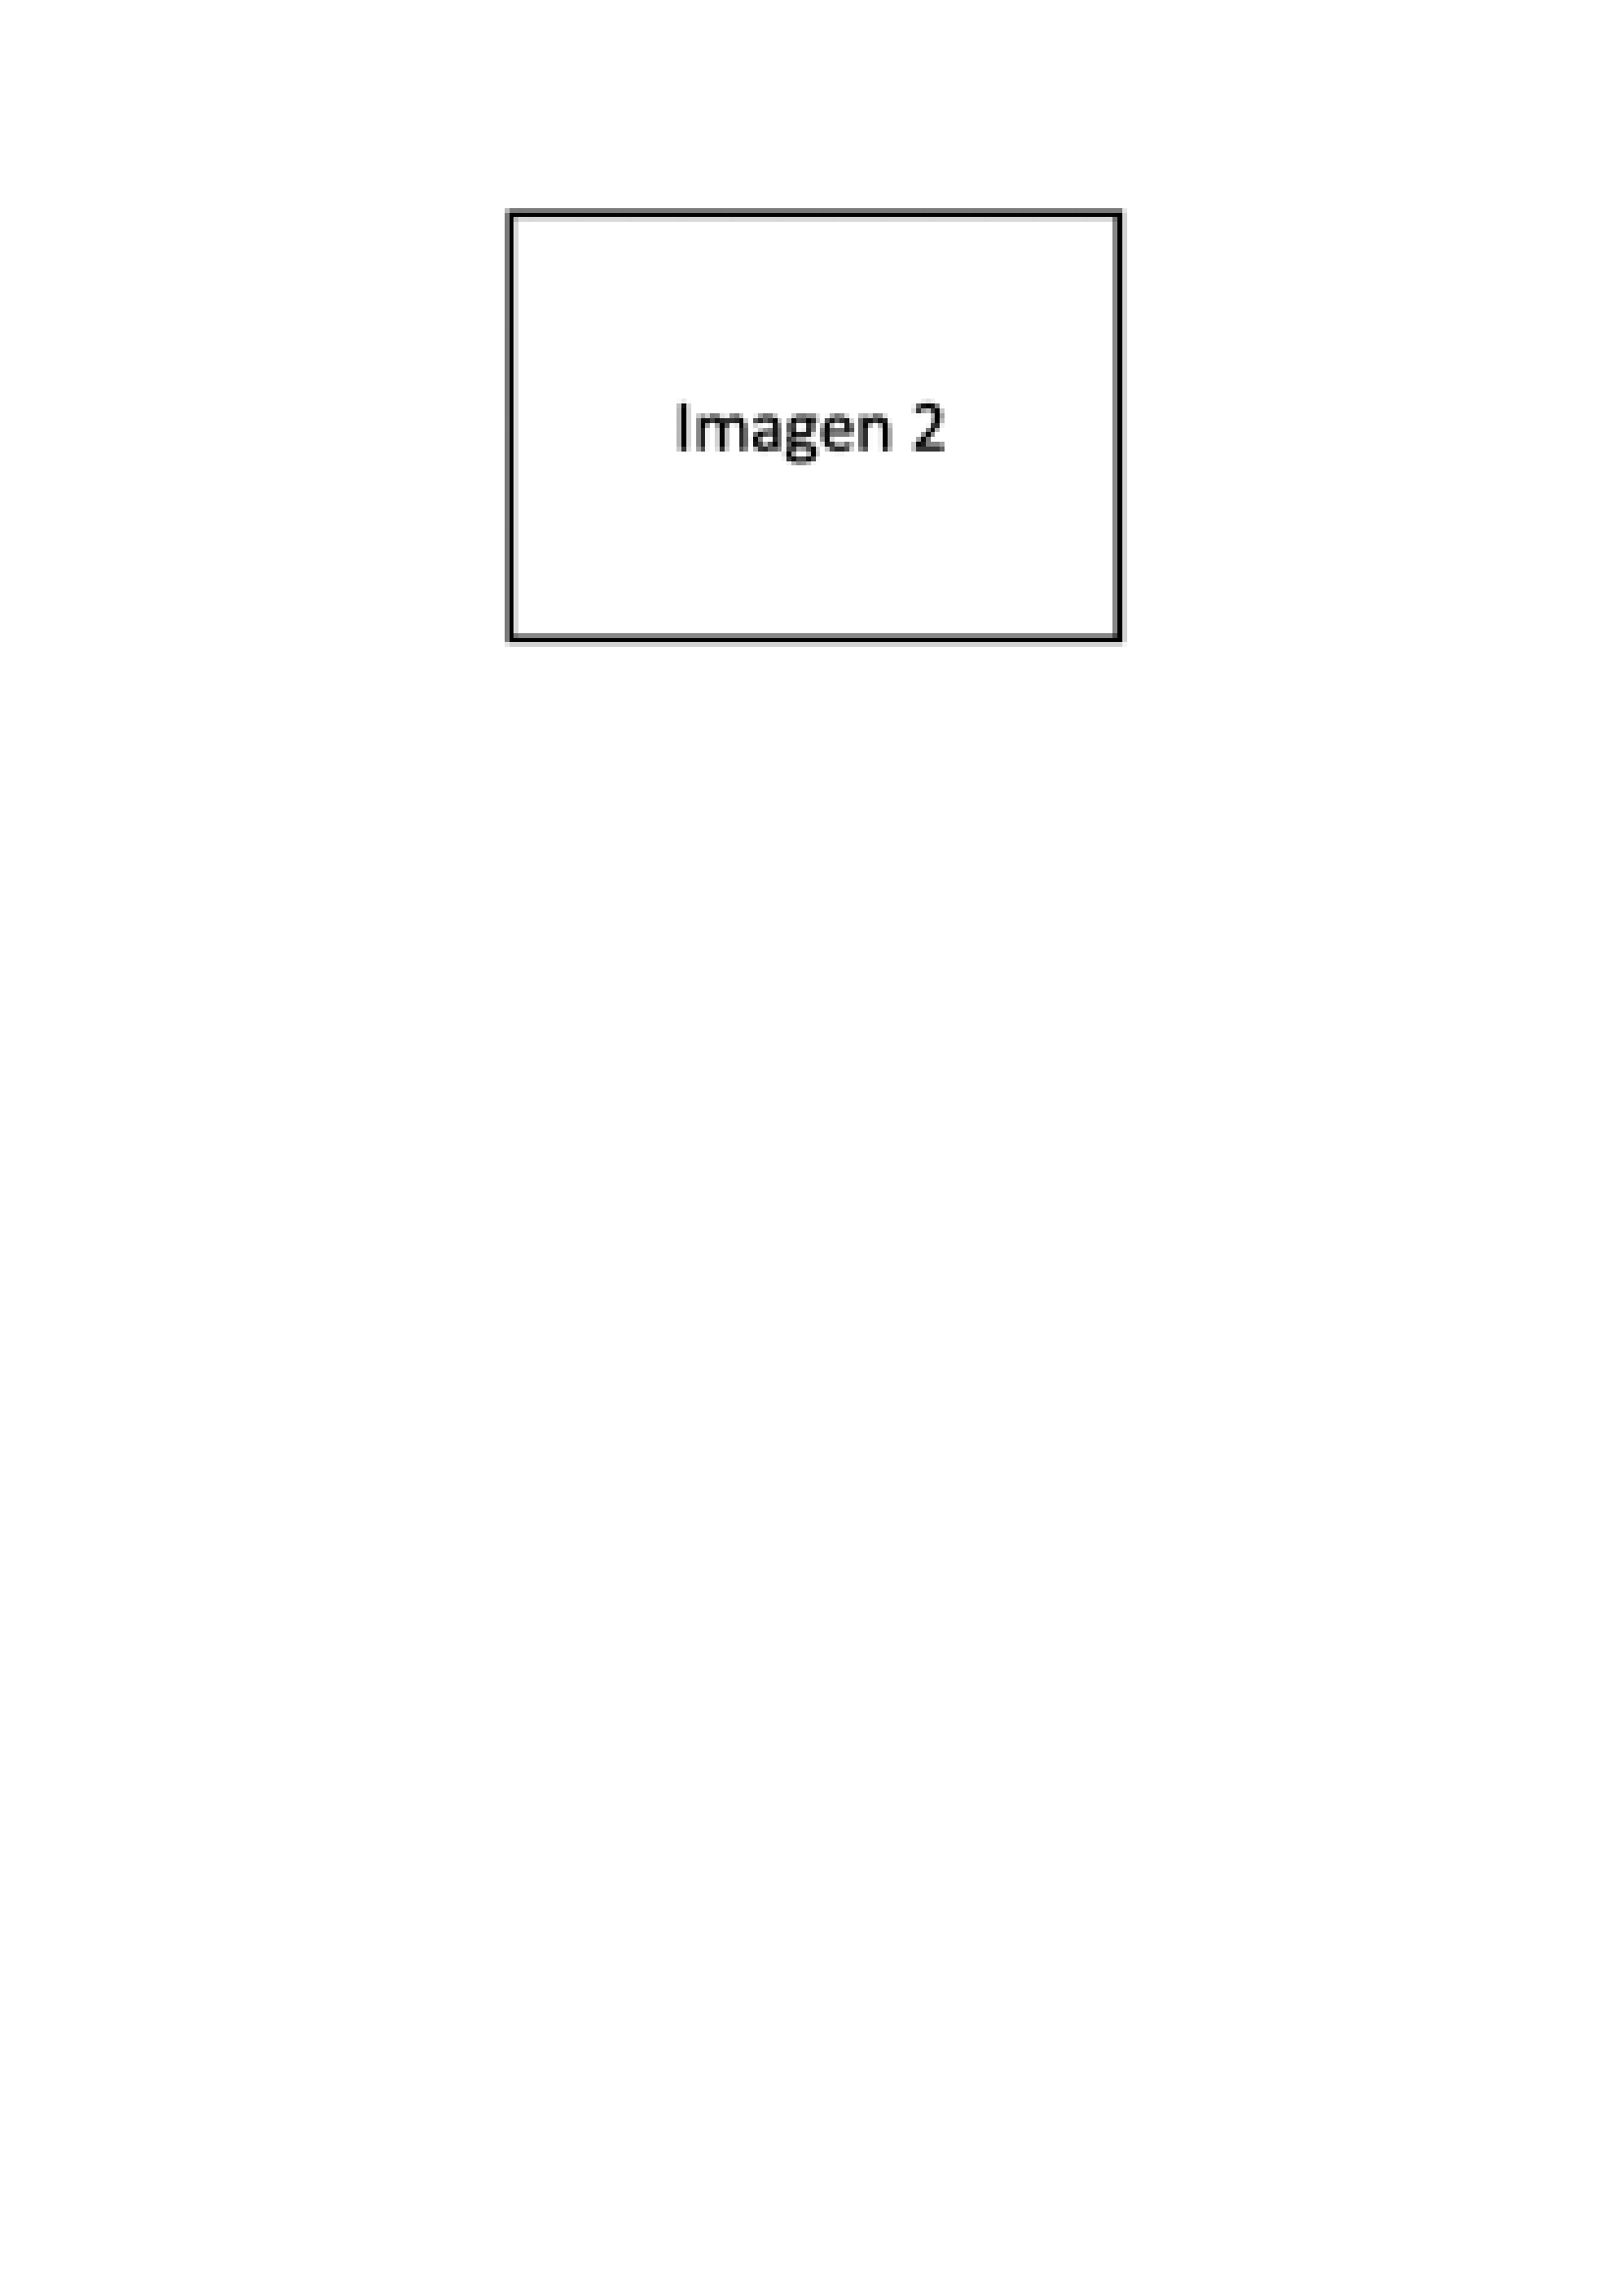
\includegraphics[scale=0.68]{secciones/imagenes/imagen2}
    \end{center}
    \caption{Ejemplo de figura. \label{imagen2}}
\end{figure}

\subsection{Título de la segunda subsección}
Contenido de la segunda subsección. Ejemplo de ecuación matemática es la ecuación 1:

\begin{equation}
    e=mc^2
    \label{ecuacion}
\end{equation}
Así se escribe Ley de Gauss para el campo magnético: %Chicharronera $x = \frac {-b \pm \sqrt {b^2 - 4ac}}{2a}$ 
\begin{align*}
        \oint_S \vec{B} \cdot d\vec{s} = 0& \qquad
\end{align*}

\subsection{Título de la tercera subsección}
Contenido de la tercera subsección. A continuación se muestra un ejemplo de elementos en viñetas:

\begin{itemize} %Ambiente o entorno itemize
    \renewcommand{\labelitemi}{\ding{42}} %dentro del entorno itemize no afecta a otras viñetas
    \renewcommand{\labelitemii}{\ding{43}} %renombrando items
    \item [+]\textit{uno.}
    \item \textbf{dos.}
    \item \underline{tres.}
    \begin{itemize}
        \item cuatro
        \begin{itemize}
            \item cinco
            \begin{itemize}
                \item ultimo subnivel permitido. %El uso de el idioma español cambia por defecto los simbolos en cada subnivel.
            \end{itemize}
        \end{itemize}
    \end{itemize}
    \item seis.
\end{itemize}


